\chapter{State of the art}
\label{chap:state-of-the-art}

\section{Chatbots}
From a user point of view, chatbots are trendy nowadays. Big companies such as \textit{Google} or \textit{Apple} are pushing to make the technology mainstream. Even if not every lambda people understand the word \say{chatbot}, they all have at least a mental representation of it. Indeed, whether they call it Digital Assistant, Siri, Ok Google, and so on, in the end, they all get the concept of an \gls{ai} narrowed to more or less human-like conversations.

\subsection{History of Chatbots}
From when are they coming? Not mentioning \textit{Alan Turing} or \textit{Joseph Weizenbaum}, considered as the fathers of \gls{ai} and chatbots, would not be fair. Indeed, they forecasted in 1950 that computers would be able to use human-like communication, and proposed a test to distinguish humans from machines, called the Turing Test\cite{paper:turing}: where a human is asked to talk to a masked entity and determine if he is talking to a human or a computer. If the human cannot determine who is the computer, then the machine passed the Turing test, as seen on figure ~\ref{fig:wikipedia_turing_test_img}. \\

In 1966, Joseph Weizenbaum wrote Eliza\cite{chatbot:eliza}, a computer program simulating a psychotherapist, seen as one of the first well-known attempts to make a Chatbot passing Turing test. Note that due to technical restrictions, Eliza is not performing well at all time. As it is for today, it is possible to play with it on a dedicated website.\\

Since Eliza, a lot of progress has been made, indeed, to only cite a few noticeable chatbots: \textit{Parry}\cite{chatbot:parry} (1972), \textit{Jabberwack}\cite{chatbot:jabberwack} (1988), \textit{Dr. Sbaitso}\cite{chatbot:dr-sbaitso} (1991), \textit{A.L.I.C.E}\cite{chatbot:alice} (1995), \textit{Smarterchild}\cite{chatbot:smarterchild} (2001), \textit{Watson}\cite{chatbot:watson} (2006), \textit{Siri}\cite{chatbot:siri} (2010), \textit{OK Google}\cite{chatbot:google} (2012), \textit{Alexa}\cite{chatbot:alexa} (2014), \textit{Cortana}\cite{chatbot:cortana} (2014), Facebook Bots\cite{chatbot:facebook} (2016), and \textit{Tay}\cite{chatbot:tay} (2016), which where all part of the Chatbot history \cite{chatbot:futurism_history_infography}.\\

From IF-ELSE, \gls{aiml}, up to \gls{ml} with \gls{ann} and \gls{dnn}, the improvements in the field of chatbots increased drastically over the years. At every iteration, the algorithms are becoming more sophisticated and better at using the human language, which is now called the field of the \gls{nlp} and \gls{nlu}.

\begin{figure}[ht!]
    \centering
    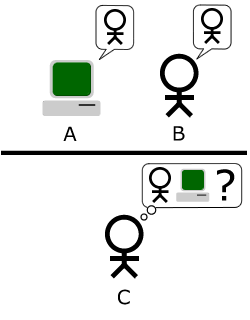
\includegraphics[width=\textwidth,height=6cm,keepaspectratio=true]{Turing_Test_version_3}
    \caption{
       Representation of the Turing Test, where user C is tasked to determine which of A or B is the computer and the human. \cite{wikipedia:turing_test_img}
    }
    \label{fig:wikipedia_turing_test_img}
\end{figure}

\subsection{Narrow Chatbots}
Once again, chatbots are almost everywhere nowadays. Indeed, it became a common tool for companies of any size to communicate with their customers and a toy for users. However, most of the time, Chatbots are not understood by their users and are leading to a high level of frustration. Even if they are becoming increasingly mainstream and sophistical, people do not realize their limits. Today's chatbots are often mistaken for \gls{agi} in \gls{scifi} and are expected to do much more than they can do. Indeed, making \gls{ani} chatbots implies a specialization into a specific field.\\

Not to forget that the primary purpose of chatbots is to provide a conversational service to the user from text to vocal or even visual format. However, its purpose can be derivated in an almost unlimited amount of solutions such as Health, Weather, Customer Service, Games, and much more.

\subsection{\gls{ir} Chatbots}
Most of the time used by \gls{faq} chatbots, which are probably the most common type of chatbots, its goal is to answer specific questions, based on a specific keyword. Indeed, the communication skills are limited to pre-made sentences and a question/answer database, which often results, in the best case scenario, in a perfect match, or the worst case scenario, in the return of something unexpected.\\

Technically speaking, \gls{ir} is part of the \gls{dm} in the field of \gls{ml}. It is well suited for search engines, as it works in a query mode. Indeed, the algorithm tries to find the best match to the submitted query in its database, usually with pattern extraction and a rank. 

\subsection{Sequential Chatbots}
\say{If he says this, then say that, then do so.}
This sentence is a good example of the concept of sequential chatbots. From a communication point of view, it does not have to talk to accomplish its purpose; it is indeed usually based on a keyword detection technic to determine what pre-made action to do. However, as the whole system works on pre-made actions, the development of such algorithms requires a lot of brain power from the developers. Indeed, as all actions result from anticipated specific keywords, and even specific order of keywords, the complexity can quickly increase, which most of the time, makes sequential chatbots seen as command line terminals instead of conversational chatbots.

\subsection{Forwarding Chatbots}
Often used by companies for customer service, it has become the most popular type of chatbots and seen as a hybridization of the \gls{ir} and sequential chatbots. Its goal is to simulate an agent that is available 24/7 to help the customer. Indeed, it will try its best to answer the most popular questions based on its \gls{faq} database and forward the user seamlessly to a human agent if its knowledge is getting limited. In the best case scenario, it is greatly appreciated by the user as the transition from Chatbot to human is not noticeable.

\subsection{Learning Chatbots} 
As \gls{ml} evolves at an incredible rate and is boosted by \gls{dnn}, new \gls{nlp} algorithms emerges, and most of the time leaves the previous generation far behind. Modern learning chatbots algorithms are what come closer to human-like conversations. Leaving the algorithm progress alone through iterations on a large dataset or commonly named \gls{bd} of real conversations, it will learn patterns by itself. However, the output generated by the trained model is dependent on the data the training occurred on. The most well-known example is \textit{Tay}\cite{chatbot:tay} (2016), the Twitter chatbot from Microsoft, that was influenced by the 4chan community to make it speak like a Young Racist Girl.\\

However, it is essential to take note that learning chatbots have been existing for a long time now. \textit{A.L.I.C.E}\cite{chatbot:alice} had already basic learning skills, as \gls{aiml} was taking care of saving variable on the run, such as the first name of the user. Even if this methodology could be seen archaic if compared to new \gls{dl} algorithms such as LSTM, it is still used today likewise the \gls{aiml} technology.


\subsection{Proactive Chatbots}
\say{Hey, I saw that you are on the website for some minutes now, do you need some more dedicated information?}. It is almost impossible that someone never received a message alike. Indeed, proactivity is not new in the field of chatbots. Mimicking an interest from the Chatbot to initiate conversations has become a standard in marketing and customer support chatbots. However, the limitations are hit fast, beyond asking general questions, not much progress has been made until now.\\

True proactive chatbots are implying that the algorithm is capable of initiating conversations from a human-like perspective, initiating the conversation or asking information in a meaningful manner based on the user, the context and the relationship with the user. The state-of-the-art search could not find any evidence of existing real proactive chatbots as described.


\subsection{Chatbot Examples}
As a help to get a feeling about narrow chatbots, a none-exhaustive list of applications is available below, and for more references about chatbots, Chatbot .org\cite{chatbot:chatbots-org} is an excellent, up to date, place about referencing old and new chatbots.

\begin{itemize}
\setlength\itemsep{0em}
\item Receive relevant information about a trip, book flights, and hotels, and get updated on the boarding and weather conditions at the airport.
\item Keep track and order coffee remotely at the office.
\item Monitor customer's satisfaction.
\item Convert potential customer into paying customers by interacting with them at the right moment.
\item Personal assistant on-the-go, get the schedule and the next meetings.
\item Relay for people on hold at a service.
\end{itemize}


\subsection{Narrow Chatbots compared to General Chatbots}
Before going further into the world of general chatbots, it is required to understand the following two axes of \gls{ai} defined by Tasks and Knowledge.
Indeed, narrow chatbots are limited by the range of tasks they can accomplish and the knowledge they can use. However, most of the time, they are very good at a particular task for a particular knowledge requirement. The table \ref{tab:agi-ani-gc} tries to represent the position of Narrow and General Chatbots on those two axes.

\vspace{1em}
\textbf{Tasks:}
Talk, \gls{faq}, Remote Control, Customer, or Placing orders are just a few tasks that a chatbot could accomplish.

\vspace{1em}
\textbf{Knowledge:}
Health, Weather, Customer Service, or Games are just a few knowledge examples chatbots could excel at.

\newcommand\MyBox[2]{
  \fbox{\lower0.75cm
    \vbox to 2cm{\vfil
      \hbox to 6cm{\hfil\parbox{5cm}{#1\\#2}\hfil}
      \vfil}
  }
}
%\noindent
%\renewcommand\arraystretch{1.5}
\setlength\tabcolsep{0pt}
\begin{table}[H]
\centering
\begin{tabular}{c >{\bfseries}r @{\hspace{0.7em}}c @{\hspace{0.4em}}c @{\hspace{0.7em}}l}
  \multirow{10}{*}{\rotatebox{90}{\parbox{5.5cm}{\bfseries\centering Tasks}}} & 
  & \multicolumn{2}{c}{\bfseries Knowledge} & \\
  & & \MyBox{Expert in a specific Field}{Expert at all Tasks} & \MyBox{\textbf{General Chatbots}\\Expert in all Fields}{Expert at all Tasks} \\[2.4em]
  & & \MyBox{\textbf{Narrow Chatbots}\\Expert in a specific Field}{Expert at specific Task} & \MyBox{Expert in all Fields}{Expert at specific Task} \\
\end{tabular}
\caption{Tasks versus Knowledge in the field of Chatbots}
\label{tab:agi-ani-gc}
\end{table}



%\begin{minipage}{\textwidth}
\subsection{General Chatbots}
\label{sota:chatbots-general}
Much effort is being made to get chatbots that can perform well simultaneously in various tasks and knowledge. Indeed, general chatbots are not limited to previously learned tasks and subjects; they should also be able to learn and relearn.\\

Those type of chatbots have not been found during the state of the art phase, and are probably by this mean either none-existant at the moment or hidden in laboratories, far from public knowledge. \\

However, big companies like Amazon are providing to the public a feel of general chatbots with \textit{Alexa}\cite{chatbot:alexa}. Users can converse with it, command their smart houses, use it as a personal assistant, and even program it to perform custom actions. However, it is not yet able to learn by itself and generate out of the blue none-programmed skills.\\

Note that general chatbots could be scary for lambda people if it starts mimicking human being too well, as in the user's mind, talking to a machine should be differentiable from talking to humans. Admittedly, in the case of the \textit{Turing Test}\cite{paper:turing}, the human does not know if it is talking to a human or a machine, which makes it probably more comfortable to accept than talking to a machine directly. \gls{scifi} is conditioning people to believe that human-like performing machines are dangerous for the human species.


\subsection{From \gls{ani} to \gls{agi}}
On a side, even if it is not part of the \gls{dp}, it is interesting to write a few lines about \gls{ai}. New incredible algorithms outperforming the previous one, and experiments reports are emerging almost every month and redefining the standard of \gls{ai}. Paradigms are shifting and technologically speaking; we are entering a new era of computer-assisted humankind.

\subsection{\gls{ani}}
More than a sequential algorithm, narrow artificial intelligence in modern terminology is the definition of \say{being good at something}. \gls{ani} has been made possible with the huge progress in \gls{ml}, the arrival of the \gls{dl}, and the need for humans to store data about everything (\gls{bd}). In medicine, for instance, it is sometimes performing so well that humans, who spent years studying, are left behind by an algorithm trained on large datasets for a few days.

\subsection{\gls{agi}}
The next step into the field of \gls{ai}, when supervision has been banned as a teaching method for algorithms as the human interaction is inputting more errors than machine themselves if unsupervised. In addition to teaching themselves, algorithms are teaching each other, and improve over the iteration with auto corrections and optimizations. They are excelling at all tasks requiring repetition, precision, and safety. Besides, they are also all able to retrieve any available information and use it for their need. \say{In the future, machines will be able to understand and do everything, much more efficiently than humans.}
%\end{minipage}


\section{\gls{nlp}}
Present in our daily lives, this technology is used massively to automate the extraction of information from human communication. In other words, it is seen as the given skill to machines to comprehend human language.

\paragraph{Examples}
The following is an non-exhaustive list of \gls{nlp} use:
\begin{itemize}
    \setlength\itemsep{0em}
    \item Customer Support Chatbots
    \item Translation into foreign languages
    \item Voice recognition
    \item Spam filters
    \item Interpreting written queries
    \item Generation of the responses
\end{itemize}

\subsection{\gls{nl}}
Naively, it is the language naturally used by humans. The goal of the \gls{nlp} is to mimic the \gls{nl} to create a human-like verbal interaction. However, it is not an easy task as it is nearly not possible to teach a machine to talk like a human. Indeed, even if machine are given the same language rules as humans, they do not understand by themselves, and are just applying the provided rules, resulting in a problem during conversational ambiguities. It would be necessary to sequentially teach the missing pieces of information, which would result in an almost an unlimited amount of conditions.

\paragraph{\gls{nl} decomposition}
Beyond the grammar and orthography, human language is composed of an incredible amount of subtleties, which makes sense most of the time intuitively for humans, but not for machines. To help understand the complexity behind \gls{nl}, the following list expresses the foundation of human language:

\begin{itemize}
    \setlength\itemsep{0em}
    \item Semantics: express the relations between words, sentences, paragraphs, etc.
    \item Morphology: maintain a structure and the content of word forms
    \item Phonology: sounds used to express words
    \item Syntax: rules applied to the bag of words to create valid texts
    \item Pragmatics: how the context influences the meaning of words
\end{itemize}



\subsection{Current \gls{nlp} technics}
Most of the following technics have been developed in the \gls{ir} field.

\begin{itemize}
    \setlength\itemsep{0em}
    \item \gls{tf-idf}: Used to set the word importance in corpora.
    \item \gls{cbow} [\ref{analyse:cbow}]: Counts the words occurrences throughout in corpus.
    \item Skip-Grams [\ref{analyse:skip-grams}]: Counts the occurrences of the character throughout in corpus.
    \item Topic modeling: Text clustering providing meaningful information to discover hidden structures via text chunking to identify the parts of the sentence in relation to each other.
    \item Segmentation: Split corpus into predefined parts, such as: \textit{sentences, paragraphs, chapters, etc.}
    \item Tokenization: Split the sentences into words.
    \item Tagging: Based on a pre-made dictionary, it gives a new layer of meaning to the word, such as: \textit{verb, adverb, noun, people name, locations, number, etc.}
    \item Dictionary: Use of tokenized words to build a dictionary, which could contain the word occurrences.
    \item Stop Words: Ignoring words only used as liaisons, and not containing information, such as: \textit{and, or, etc.}
    \item Stemming: Uniformizing words to their root by removing the prefix and suffix, such as: \textit{remake and loveable}.
    \item Lemmatization: Replace the words to their base form, such as \textit{conjugated verb}.
\end{itemize}

\subsection{\gls{nlp} declensions}
Further into the field of \gls{nlp}, it is today commonly split into two groups:

\paragraph{\gls{nlu}}
It is a subdivision of \gls{dm}, and it involves the processing of the text by analyzing its content by extracting relevant information, usually called keywords.

\paragraph{\gls{nlg}}
In combination with \gls{nlu}, often applied to text classification, \gls{nlg} is useful to generate custom sentences, using custom keyword extracted to make the response to a query even more relevant and usually keeps track of the context.


\section{Word Embedding}
\label{stoa:word-embedding}
It can be summarised as the vector representation of a word and often using between 100 and 400 dimensions. Its position in the multi-dimensional space keeps track of the word context and semantic to a dictionary of words and the corpora. Due to the vector nature of the words, geometrical operations can be applied to those words to find word similarities and relationship between them. 


\subsection{Word2Vec}
\label{stoa:word2vec}
Published by Google in 2013, Word2Vec\cite{article:word2vec}, probably became, the most popular algorithm in the word embedding field, nowadays. It uses a \gls{snn} ~\ref{fig:wikipedia_colored_neural_network_img}, similar to a conventional supervised model. Indeed, it is a two-layer \gls{nn}, its input is text corpora, and its output is word vectors based on a given dictionary. Even if it is easy to train and test, it is often difficult to tweak the algorithm, and as a result, makes it harder to make a good generalization. Even if it is not using \gls{dl} itself as output, the input text form of the words are transformed into their value form, which makes it incredibly powerful and useful for \gls{dnn} algorithms as input.

\begin{figure}[ht!]
    \centering
    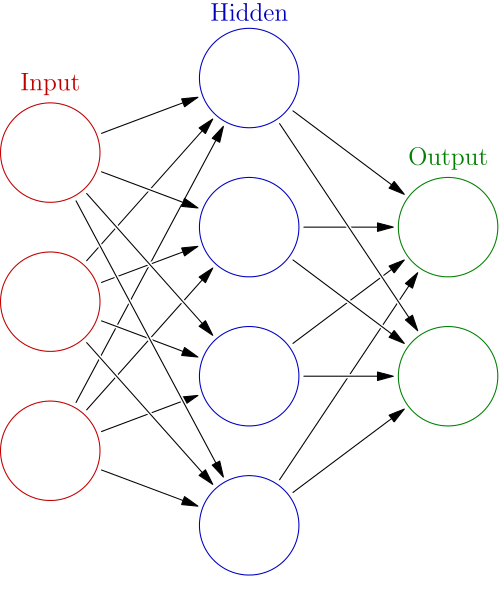
\includegraphics[width=\textwidth,height=6cm,keepaspectratio=true]{500px-Colored_neural_network}
    \caption{
       Artificial neural network with layer coloring \cite{wikipedia:colored_neural_network_img}
    }
    \label{fig:wikipedia_colored_neural_network_img}
\end{figure}


\subsection{Gensim Framework}
\label{stoa:gensim}
Since its publication in 2013, Word2Vec\cite{article:word2vec} various actors implemented the algorithm and companies like RaRe Technologies\cite{company:rare-technologies}, specialized in \gls{nlp}, made it easier for Scientist and Hobbyists to jump right in. Which probably influenced its popularity by making it accessible for the community instead of big companies and institutions only. In the case of this \gls{dp}, the author will be focusing on the framework made available by RaRe Technologies and more specifically by RaRe Consulting\cite{company:rare-consulting}, Gensim\cite{article:rehurek_lrec}. Other frameworks and solutions are available, they are in the end implementing the same algorithm generating a Word2Vec model by capturing the context of the words, but they are different by their language and their different integration with custom features.\\

Gensim is a python implementation of Word2Vec, and it is not a general purpose \gls{ml} or even \gls{dl} framework. However, in order of magnitude, it does one thing, but does it very well, as it does its job faster that Tensorflow\cite{article:tensorflow2015-whitepaper} for instance.

\section{Word2Vec Alternatives}
Word2Vec does not define Word Embedding; indeed the concept of the vector representation in a multi-dimensional space has multiple solutions to it. Without going into too many details, and to name a few, the following could be alternatives to Word2Vec, with their pros and cons.

\subsection{Word2Vec\cite{article:word2vec}}
\label{stoa:word2vec-pros-cons}
With the purpose to make the following alternatives comparable, the following are the pros and cons for Word2Vec itself.
\paragraph{Pros}
\begin{itemize}
    \setlength\itemsep{0em}
    \item First word embedding solution to be able to generate a model on a large corpus with a dictionary containing millions of words.
    \item Outputs word vectors based on corpora with raw text.
\end{itemize}
\paragraph{Cons}
\begin{itemize}
    \setlength\itemsep{0em}
    \item Difficulties to extract the sense of words with multiple meanings depending on the context. e.g., the word \textbf{Doctor}, it could be the Academic Title, a Physician, or even the name of a TV-Show.
\end{itemize}

\subsection{FastText\cite{article:fasttext}}
Made by Facebook.
\paragraph{Pros}
\begin{itemize}
    \setlength\itemsep{0em}
    \item Same as Word2Vec, except that technically it use the Skip-Grams [\ref{analyse:skip-grams}] technics to train on characters composing the words instead of \gls{cbow} [\ref{analyse:cbow}], which traines with words.
\end{itemize}
\paragraph{Cons}
\begin{itemize}
    \setlength\itemsep{0em}
    \item Same as Word2Vec, words with multiple meanings are not managed well.
\end{itemize}


\subsection{Glove\cite{article:glove}}
Global Vectors for Word Representation is a contribution to the Word Embedding by the University of Standford in \gls{nlp}.
\paragraph{Pros}
\begin{itemize}
    \setlength\itemsep{0em}
    \item Less time consuming than Word2Vec.
    \item Depending on the scenario and benchmarks, it sometimes performs better than Word2Vec at tasks related to semantic.
\end{itemize}
\paragraph{Cons}
\begin{itemize}
    \setlength\itemsep{0em}
    \item Larger memory usage than Word2Vec.
    \item Same as Word2Vec for multiple word meanings.
\end{itemize}


\subsection{Adagram\cite{article:adagram}}
\label{sec:adagram}
Adaptive Skip-Gram is a Russian contribution by National Research University of Moscow.
\paragraph{Pros}
\begin{itemize}
    \setlength\itemsep{0em}
    \item It claims, contrary to Word2Vec, to be able to manage different word meanings as it should extract the context of the surrounding words.
\end{itemize}
\paragraph{Cons}
\begin{itemize}
    \setlength\itemsep{0em}
    \item In the current state, it is not designed for corpora with a dictionary larger than tens of millions of words.
    \item Does not keep track of the word order.
\end{itemize}


\section{Word Embedding Extensions}
Based on the Word Embedding technics, proposals were raised about its extension to the sentences and even documents. A simple solution to generate a sentence/documents representation would be to sum word vectors composing the sentences/documents; however, the following non-exhaustive technics are performing better than naive addition.

\subsection{Doc2vec\cite{article:doc2vec}}
Adaptation of Word2Vec for document embedding.
\paragraph{Pros}
\begin{itemize}
    \setlength\itemsep{0em}
    \item Based on Word2Vec.
    \item Performs well in most cases.
\end{itemize}
\paragraph{Cons}
\begin{itemize}
    \setlength\itemsep{0em}
    \item In few cases the embedding could be biased towards the specific content words.\cite{article:doc2vec_eval}
\end{itemize}

\subsection{Skip-thought\cite{article:skip-thought}}
Made for corpus with semantically related sentences.
\paragraph{Pros}
\begin{itemize}
    \setlength\itemsep{0em}
    \item Works well with corpus having a sentence continuity.
\end{itemize}
\paragraph{Cons}
\begin{itemize}
    \setlength\itemsep{0em}
    \item Adjacent sentences must be semantically related.
\end{itemize}

\subsection{RNN}
\label{sota:rnn}
With the current market and institutional need to make everything \gls{dl}, the subject of \gls{dnn} must be slightly overviewed. All the technics described previously in this chapter are not using \gls{dnn}, and there is a good reason for their success. Indeed, they do not require labeled data for training, which is required by \gls{dl} algorithms. However, the idea has not been abandoned; solutions are raising to overcome this drawback, such as using crowd-based solution, which uses users as signals to determine document similarities \cite{article:lstm-deep-sentence-embedding}.



\section{Beyond Word Embedding}
As \gls{nlp} usage increases over the years, Word Embedding technics and its extensions are becoming increasingly more sophisticated and are getting closer to human-like generalization. As controversially suggested by Geoffrey Hinton, famous \gls{dl} researcher, it would be possible to get to human-like conversational capabilities via a method he calls Thought Vectors \cite{article:thought2vec-geoffrey-hinton}. Without going into exciting details, it implies for the \gls{agi}, at this stage, even if the algorithm does not understand the meaning of the sentences, the reasoning behind a thought would be well enough emulated to make it human-like.

\subsection{Though Embedding}
\label{sota:though-embedding}
A vectorized thought would be trained to generate a thought's context. As for Word Embedding and Doc Embedding,  Thought Embedding are linked by a chain of reasoning.

\subsection{Contextual embeddings}
\label{sota:contextual-embedding}
Thought Embedding paper and implementation is yet to be made, however, progress has been made in this direction with contextual embeddings Context2Vec\cite{article:context2vec}. It is a bidirectional LSTM\cite{article:lstm} unsupervised model generating a Word Embedding based on its occurrence in the sentences, which unlike Adagram[\ref{sec:adagram}] is taking into account order. \\


However, Context2Vec does not define Contextual Embeddings. New emerging 2019 algorithms, based on the attention mechanism \cite{article:attention-is-all-you-need}, such as Transformers\cite{article:transformer} or even further its bidirectional extension BERT\cite{article:bert}, which makes LSTM almost obsolete.

\paragraph{Summarized}
\begin{itemize}
    \setlength\itemsep{0em}
    \item Context dependent word embeddings.
    \item Can generate sentence embeddings.
    \item The output can be used almost as it is for NLP.
    \item Tracking using selective "forget" gates.
\end{itemize}


\section{Datasets}
\label{sota:datasets}
Nowadays, in data engineering, the new gold is data. Luckily, today is driven by \gls{bd}, and almost any kind of data is available to who knows where to look at. For the case of the \gls{dp}, the author is interested in conversational data. Even though the English Wikipedia Dump from 09th May 2019 will be using exclusively, the following is a non-exhaustive list of corpora gathered during the \gls{dp}.

\begin{itemize}
    \setlength\itemsep{0em}
    \item Wikipedia Dumps Index: \url{https://dumps.wikimedia.org/backup-index.html}
    \item English Wikipedia Dumps (bzip2: 16Gb, raw: 90Gb): \url{https://dumps.wikimedia.org/enwiki/latest/} [enwiki-latest-pages-articles.xml.bz2]
    \item Reddit Comments (bzip2: 6Gb, raw: 32Gb): \url{https://www.reddit.com/r/datasets/comments/3bxlg7/i_have_every_publicly_available_reddit_comment/}
    \item The Open American National Corpus: \url{http://www.anc.org}
    \item Santa Barbara Corpus of Spoken American English: \url{https://www.linguistics.ucsb.edu/research/santa-barbara-corpus}
    \item Leipzig Corpora Collection \url{http://wortschatz.uni-leipzig.de/en/download/}
    \item Legal Case Reports: \url{http://archive.ics.uci.edu/ml/datasets/Legal\+Case\+Reports}
    \item Cornell Newsroom: \url{https://summari.es}
    \item DeepMind Q\&A: \url{https://cs.nyu.edu/\~kcho/DMQA/}
    \item Large Movie Review: \url{http://ai.stanford.edu/\~amaas/data/sentiment/}
    \item Project Gutenberg - Free eBooks: \url{https://www.www.gutenberg.org}
\end{itemize}


\section{Word2Vec Models}
\label{sota:word2vec-models}
Training own models are very resource consumptive, and often the resources are not available, would it be datasets or computer power. Luckily, big companies like Google did the work for us, and pre-trained models that could be used out of the box. The following is a non-exhaustive list of models for Word2Vec:

\begin{itemize}
    \setlength\itemsep{0em}
    \item Gensim directory: \url{https://github.com/RaRe-Technologies/gensim-data/releases}
    \item Fasttext: \url{https://fasttext.cc/docs/en/english-vectors.html}
    \item estnltk: \url{http://ats.cs.ut.ee/keeletehnoloogia/estnltk/word2vec/}
\end{itemize}
